% 	Name		:: 	BDEEP template is based on the sthlm theme (Mark Hendry Olson (mark@hendryolson.com))
%	Author		:: 	Peter Christensen
%	Created		::	2016-04-12
%	Updated		::	June 18, 2015 at 08:45
%	Version		:: 	1.0
%	Email		:: 	pchrist@illinois.edu
%	Website		:: 	bdeep webiste
%
% 	License		:: 	This file may be distributed and/or modified under the
%                  	GNU Public License.
%
%	Description	::	This template makes use of the Stockholm theme from Mark Hendry Olson and includes items and files necessary for creating presentations on behalf of our group.


%-=-=-=-=-=-=-=-=-=-=-=-=-=-=-=-=-=-=-=-=-=-=-=-=
%
%        LOADING DOCUMENT
%
%-=-=-=-=-=-=-=-=-=-=-=-=-=-=-=-=-=-=-=-=-=-=-=-=

\documentclass[newPxFont]{beamer}
\usetheme{sthlm}
%\usecolortheme{sthlmv42}

%-=-=-=-=-=-=-=-=-=-=-=-=-=-=-=-=-=-=-=-=-=-=-=-=
%        LOADING PACKAGES
%-=-=-=-=-=-=-=-=-=-=-=-=-=-=-=-=-=-=-=-=-=-=-=-=
\usepackage[utf8]{inputenc}

\usepackage{chronology}

\renewcommand{\event}[3][e]{%
  \pgfmathsetlength\xstop{(#2-\theyearstart)*\unit}%
  \ifx #1e%
    \draw[fill=black,draw=none,opacity=0.5]%
      (\xstop, 0) circle (.2\unit)%
      node[opacity=1,rotate=45,right=.2\unit] {#3};%
  \else%
    \pgfmathsetlength\xstart{(#1-\theyearstart)*\unit}%
    \draw[fill=black,draw=none,opacity=0.5,rounded corners=.1\unit]%
      (\xstart,-.1\unit) rectangle%
      node[opacity=1,rotate=45,right=.2\unit] {#3} (\xstop,.1\unit);%
  \fi}%

%-=-=-=-=-=-=-=-=-=-=-=-=-=-=-=-=-=-=-=-=-=-=-=-=
%        BEAMER OPTIONS
%-=-=-=-=-=-=-=-=-=-=-=-=-=-=-=-=-=-=-=-=-=-=-=-=

\setbeameroption{show notes}

%-=-=-=-=-=-=-=-=-=-=-=-=-=-=-=-=-=-=-=-=-=-=-=-=
%
%	PRESENTATION INFORMATION
%
%-=-=-=-=-=-=-=-=-=-=-=-=-=-=-=-=-=-=-=-=-=-=-=-=

\title{Title of Presentation}
\subtitle{Subtitle of Presentation}
\date{today's date}
\author{your name}
\institute{University of Illinois}


\begin{document}

%-=-=-=-=-=-=-=-=-=-=-=-=-=-=-=-=-=-=-=-=-=-=-=-=
%
%	TITLE PAGE
%
%-=-=-=-=-=-=-=-=-=-=-=-=-=-=-=-=-=-=-=-=-=-=-=-=

\maketitle

%\begin{frame}[plain]
%	\titlepage
%\end{frame}

%-=-=-=-=-=-=-=-=-=-=-=-=-=-=-=-=-=-=-=-=-=-=-=-=
%
%	TABLE OF CONTENTS: OVERVIEW
%
%-=-=-=-=-=-=-=-=-=-=-=-=-=-=-=-=-=-=-=-=-=-=-=-=

\section*{Introduction}

%-=-=-=-=-=-=-=-=-=-=-=-=-=-=-=-=-=-=-=-=-=-=-=-=
%	FRAME: Introduction
%-=-=-=-=-=-=-=-=-=-=-=-=-=-=-=-=-=-=-=-=-=-=-=-=

\begin{frame}[c]{Introduction}

\begin{enumerate}
\item{First Item}   
\item{Second Item}  
\item{Third Item}
\end{enumerate}

\end{frame}



\section*{Overview}
\begin{frame}{Overview}
% For longer presentations use hideallsubsections option
\tableofcontents[hideallsubsections]
\end{frame}


%-=-=-=-=-=-=-=-=-=-=-=-=-=-=-=-=-=-=-=-=-=-=-=-=
%
%	SECTION: BACKGROUND
%
%-=-=-=-=-=-=-=-=-=-=-=-=-=-=-=-=-=-=-=-=-=-=-=-=

\section{Background}

%-=-=-=-=-=-=-=-=-=-=-=-=-=-=-=-=-=-=-=-=-=-=-=-=
%	FRAME: Slide with Graphic/Text
%-=-=-=-=-=-=-=-=-=-=-=-=-=-=-=-=-=-=-=-=-=-=-=-=
\begin{frame}[c]{Slide with Graphic/Text}
\begin{figure}
	\centering
	\includegraphics[width=0.65\linewidth]{Importer.png}
\end{figure}
\begin{enumerate}  
	\item{point #1}
	\item{point #2}  
\end{enumerate}  
\end{frame}

%-=-=-=-=-=-=-=-=-=-=-=-=-=-=-=-=-=-=-=-=-=-=-=-=
%	FRAME: Slide with Graphic Column and Text Column
%-=-=-=-=-=-=-=-=-=-=-=-=-=-=-=-=-=-=-=-=-=-=-=-=
\begin{frame}[c]{Slide with Graphic Column and Text Column}
	\begin{columns}
		\begin{column}{.68\linewidth}
			\begin{enumerate}   
				\item{First Item}
				\begin{itemize}  
					\item{first subitem}
					\item{second subitem}
					\item{third subitem}
				\end{itemize}  
			\end{enumerate}
		\end{column}
		\begin{column}{.3\linewidth}
			\begin{figure}
				\centering
				
\includegraphics[width=0.9\linewidth]{Brown.png}
			\end{figure}
		\end{column}
	\end{columns}
\end{frame}


%-=-=-=-=-=-=-=-=-=-=-=-=-=-=-=-=-=-=-=-=-=-=-=-=
%	FRAME: Slide with Items and Subitems
%-=-=-=-=-=-=-=-=-=-=-=-=-=-=-=-=-=-=-=-=-=-=-=-=
\begin{frame}[c]{Slide with Items and Subitems}
	Heading	
	\begin{enumerate}   
		\item{First Item}  
		\begin{itemize}
			\item{first subitem}
		\end{itemize}
		\item{Second Item}
		\begin{itemize}
			\item{second subitem}
		\end{itemize}
		\item{Third Item}
		\begin{itemize}
			\item{third subitem}
		\end{itemize}
	\end{enumerate}	
\end{frame}

%-=-=-=-=-=-=-=-=-=-=-=-=-=-=-=-=-=-=-=-=-=-=-=-=
%
%	SECTION: DATA AND METHODOLOGY
%
%-=-=-=-=-=-=-=-=-=-=-=-=-=-=-=-=-=-=-=-=-=-=-=-=

\section{Data and Method}
%-=-=-=-=-=-=-=-=-=-=-=-=-=-=-=-=-=-=-=-=-=-=-=-=
%	FRAME: Slide with Itemized Text and Graphics Columns
%-=-=-=-=-=-=-=-=-=-=-=-=-=-=-=-=-=-=-=-=-=-=-=-=
\begin{frame}[c]{Slide with Itemized Text and Graphics Columns}
	\begin{columns}
		\begin{column}{.6\linewidth}
			\begin{figure}
				\centering
				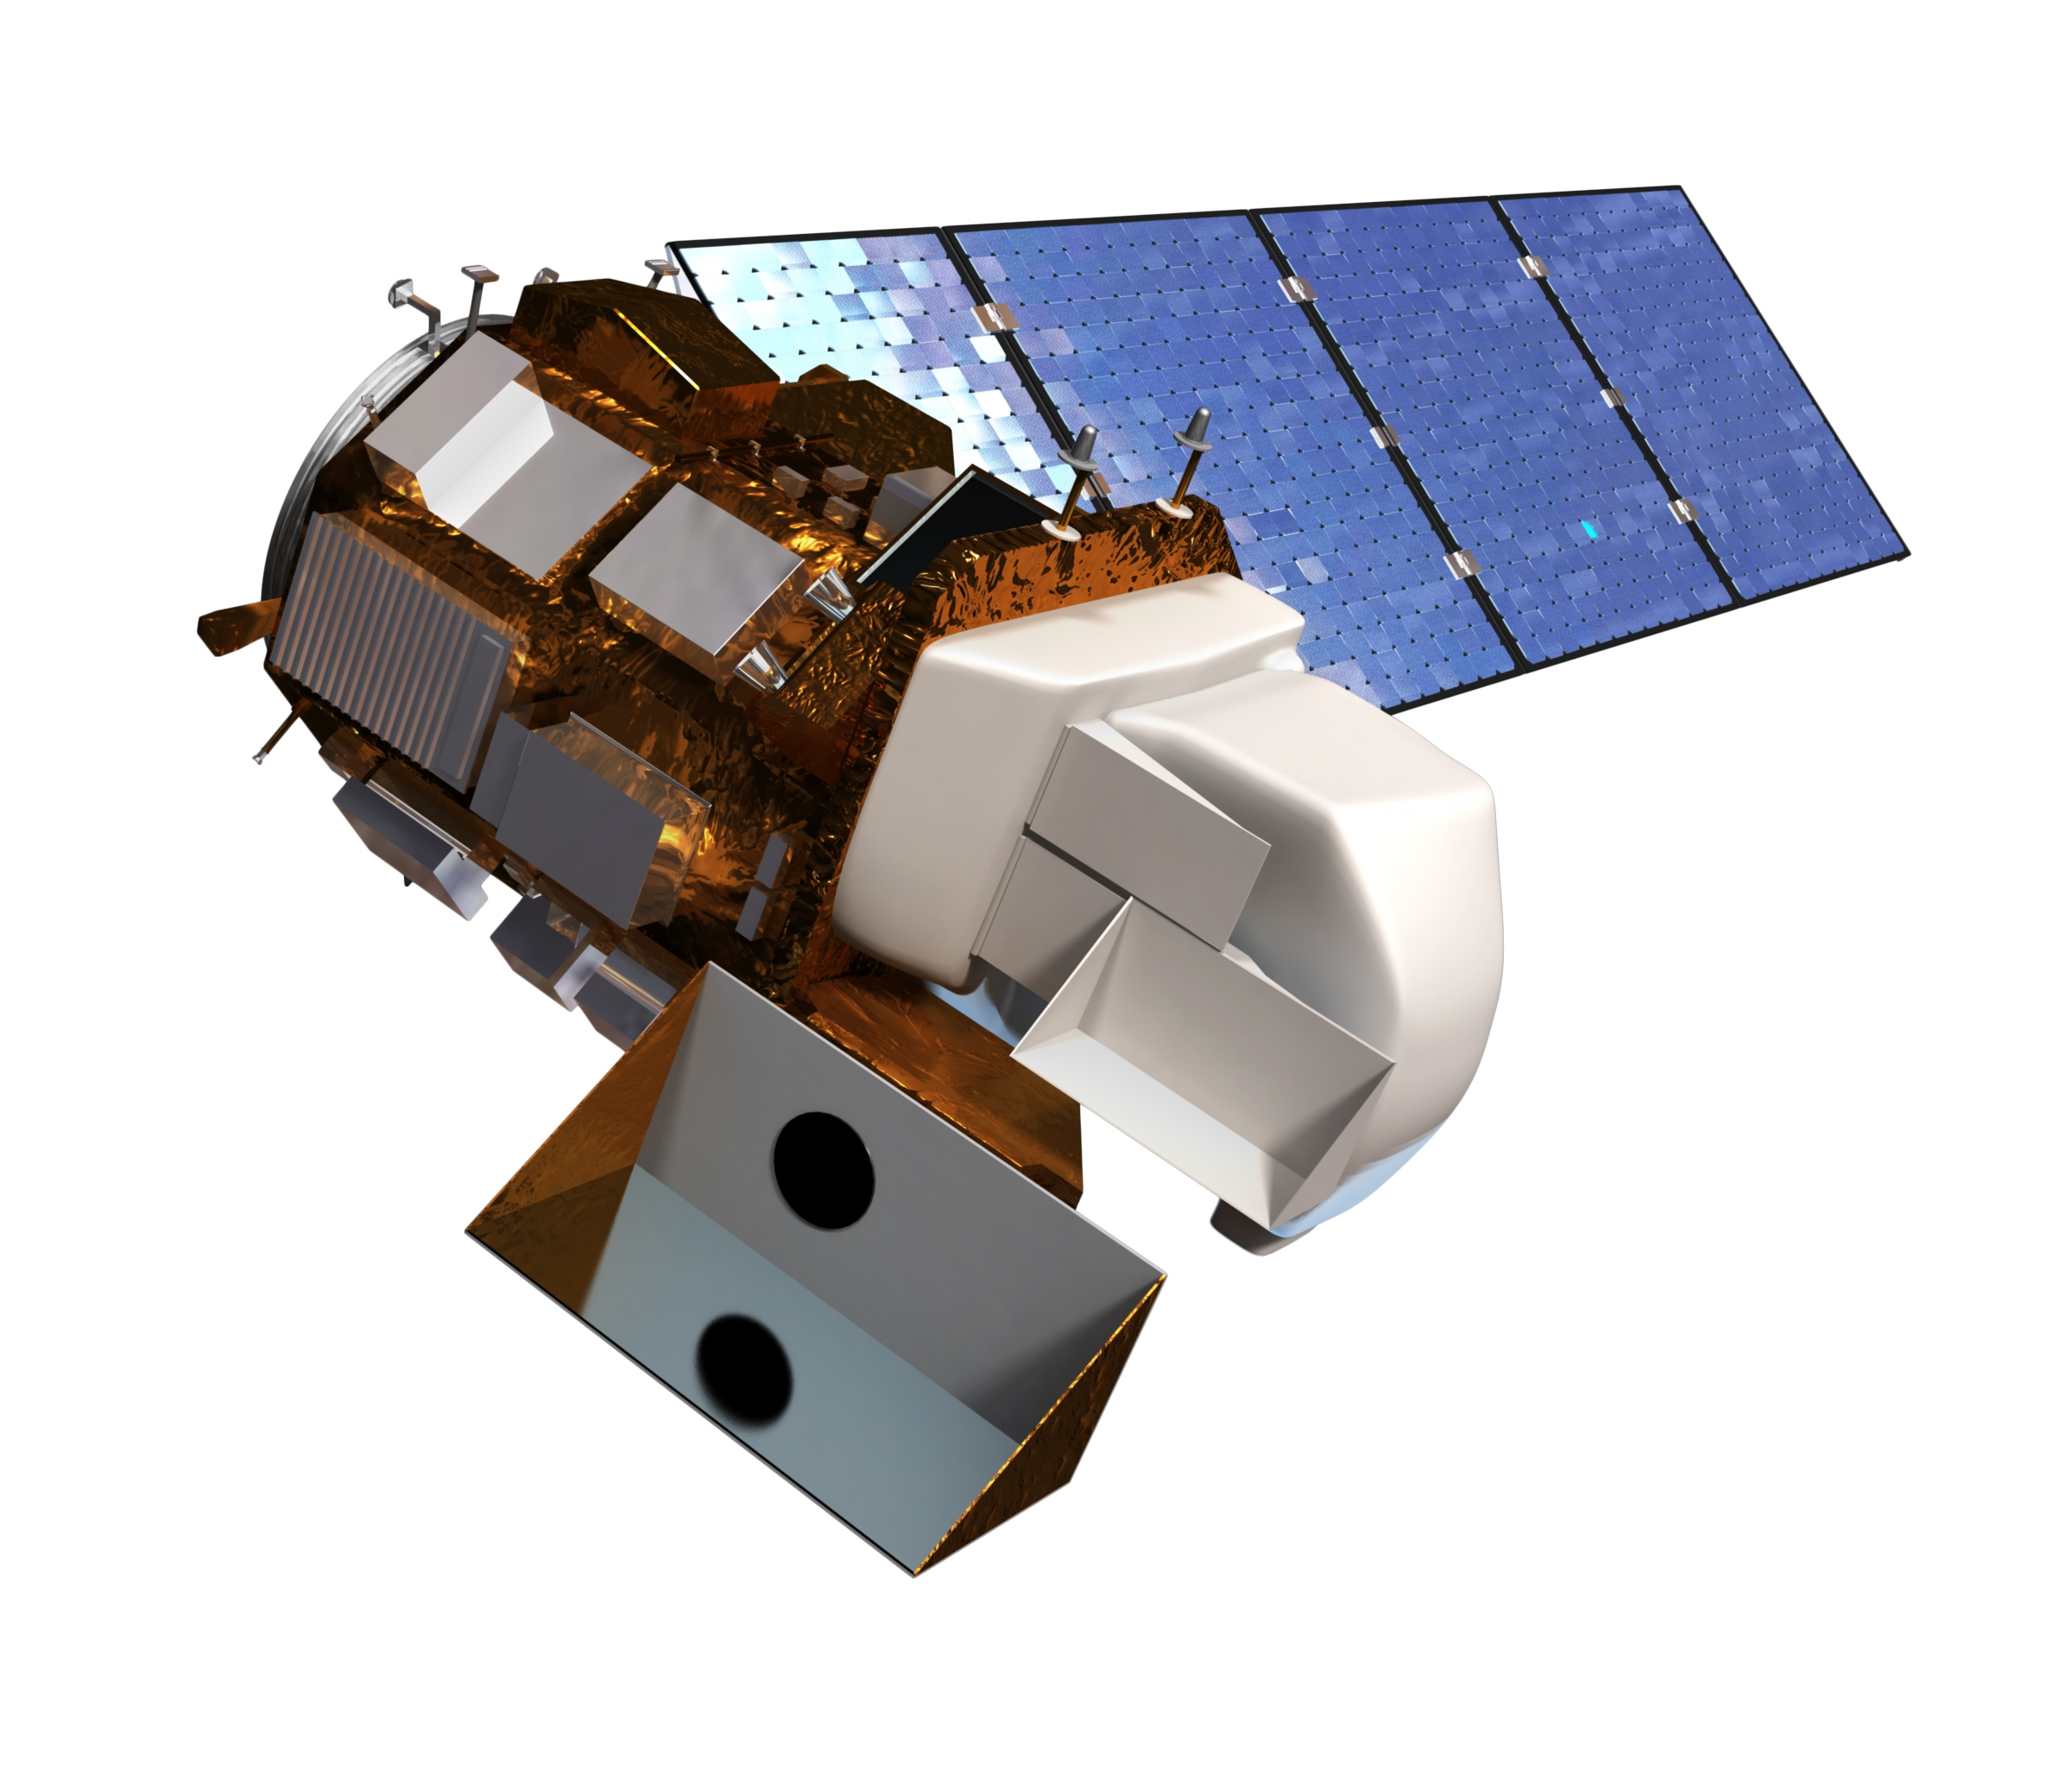
\includegraphics[width=0.4\linewidth]{Landsat8.jpg}
			\end{figure}
	\begin{itemize}
		\item{First Item}\\
		\item{Second Item}\\
		\item{Third Item}\\
	\end{itemize}
		\end{column}
		\begin{column}{.6\linewidth}
			\begin{figure}
				\centering
				\includegraphics[width=.8\linewidth]{CompareHighestResi.eps}
			\end{figure}
		\end{column}
	\end{columns}
\end{frame}


%-=-=-=-=-=-=-=-=-=-=-=-=-=-=-=-=-=-=-=-=-=-=-=-=
%	FRAME: Slide with Equations and Text
%-=-=-=-=-=-=-=-=-=-=-=-=-=-=-=-=-=-=-=-=-=-=-=-=
\begin{frame}{Slide with Equations and Text}
	Equation 1
	\begin{equation}{\label{eq1}}
	V_{i,t}^{u}-(\sum\limits_{T=0}^{\infty}V_{i,t+T}^{a})\delta^{T}-C_{t}^{a}>0   
	\end{equation}
	Text pertaining to euqation 1 with imbedded notation: ($C^{\tau}$).
	\begin{equation}{\label{eq2}}
	L_{it}^{u}=f(V_{it}^{a},C_{it}^{a},C^{\tau})
	\end{equation}
\end{frame}

%-=-=-=-=-=-=-=-=-=-=-=-=-=-=-=-=-=-=-=-=-=-=-=-=
%	FRAME: Slide with Text, Equation, and Figure/Graphic
%-=-=-=-=-=-=-=-=-=-=-=-=-=-=-=-=-=-=-=-=-=-=-=-=

\begin{frame}{Slide with Text, Equation, and Figure/Graphic}
	Equation #1:
	\begin{equation}{\label{eq2}}
		\tau_{ATT(\frac{da}{du})}=[\frac{dL^{a}}{dL^{u}}_{it}(1)-\frac{dL^{a}}{dL^{u}}_{it}(0)]
	\end{equation}
	\begin{figure}
		\centering
		\includegraphics[width=0.6\linewidth, trim=0 0 0 400, clip]{CompareHiRes_Guangzhou.eps}
	\end{figure}
\end{frame}

%-=-=-=-=-=-=-=-=-=-=-=-=-=-=-=-=-=-=-=-=-=-=-=-=
%	FRAME: Slide with Annotated Timeline
%-=-=-=-=-=-=-=-=-=-=-=-=-=-=-=-=-=-=-=-=-=-=-=-=


\begin{frame}[c]{Slide with Annotated Timeline}
	\vspace{-1cm}
	\begin{center}\begin{chronology}[5]{1988}{2005}{0.85\textwidth}
			\event[\decimaldate{1}{1}{1990}]{\decimaldate{1}{11}{1994}}{\cRed{Period 1 in red}}
			\event[\decimaldate{1}{3}{1995}]{\decimaldate{1}{11}{1999}}{ 1997 - No Net Loss Regulation}
			\event[\decimaldate{1}{3}{2000}]{\decimaldate{1}{1}{2005}}{\cRed{Period 2 in red}}
		\end{chronology}
	\end{center}
	
\end{frame}


%-=-=-=-=-=-=-=-=-=-=-=-=-=-=-=-=-=-=-=-=-=-=-=-=
%
%	SECTION: RESULTS
%
%-=-=-=-=-=-=-=-=-=-=-=-=-=-=-=-=-=-=-=-=-=-=-=-=
\section{Results}

%-=-=-=-=-=-=-=-=-=-=-=-=-=-=-=-=-=-=-=-=-=-=-=-=
%	FRAME: Results-Type Slide
%-=-=-=-=-=-=-=-=-=-=-=-=-=-=-=-=-=-=-=-=-=-=-=-=

\begin{frame}[c]{Results-Type Slide}
	Primary Findings	
	\begin{enumerate}   
		\item{First Item}
		\begin{itemize}
			\item{first subitem}
			\item{second subitem (remember that percentages must be coded correctly 50\%).}
			\item{third subitem}
			\item{fourth subitem}
		\end{itemize}
	\end{enumerate}	
\end{frame}

%-=-=-=-=-=-=-=-=-=-=-=-=-=-=-=-=-=-=-=-=-=-=-=-=
%
%	SECTION: CONCLUSIONS
%
%-=-=-=-=-=-=-=-=-=-=-=-=-=-=-=-=-=-=-=-=-=-=-=-=
\section{Conclusions}

%-=-=-=-=-=-=-=-=-=-=-=-=-=-=-=-=-=-=-=-=-=-=-=-=
%	FRAME: Conclusions
%-=-=-=-=-=-=-=-=-=-=-=-=-=-=-=-=-=-=-=-=-=-=-=-=

\begin{frame}[c]{Conclusions}
	Heading
	\begin{enumerate}   
		\item{Item 1}  
		\begin{itemize}
			\item{subitem 1}
			\item{subitem 2}
			\item{subitem 3}
		\end{itemize}
		\item{Item 2}
		\begin{itemize}
			\item{subitem 1}
			\item{subitem 2}
			\item{subitem 3}
		\end{itemize}
	\end{enumerate}	
\end{frame}

%-=-=-=-=-=-=-=-=-=-=-=-=-=-=-=-=-=-=-=-=-=-=-=-=
%
%	SECTION: LINKS AND ACKNOWLEDGEMENTS
%
%-=-=-=-=-=-=-=-=-=-=-=-=-=-=-=-=-=-=-=-=-=-=-=-=

\begin{frame}{Links and Acknowledgements}
	
You can find publications at \url{www.peterchristensen.net}.\\
\vspace{1em}
If you are interested in learning about the technology that we are building to support our economics and policy research, please come find us on the 3rd floor of the National Center for Supercomputing Applications (NCSA).\\
\vspace{1em}	
Please send questions and comments to: pchrist@illinois.edu
\end{frame}

\end{document}
